\documentclass[10pt,letterpaper]{article}

\usepackage[font=footnotesize]{caption}
\usepackage{float}
\usepackage{epsf}
\usepackage{epsfig}
\usepackage{subfigure}
% \usepackage{subfig}
\usepackage{latexsym}
%\usepackage{algorithm}
%\usepackage[noend]{algorithmic}
% \usepackage{color}
\usepackage{color, colortbl}
\usepackage{wrapfig}
\usepackage{topcapt}
\usepackage{multirow}
\usepackage{tabularx}
\usepackage{hyperref}
\usepackage{xcolor}
\usepackage{mdwlist}
\usepackage{pdfpages} 
\usepackage{xspace}

%\usepackage{color}
\newcommand{\lc}[1]{\textcolor{blue}{#1}}


\usepackage{amsmath, amsfonts, amssymb}
\usepackage[hmargin=1in,vmargin=1.2in]{geometry}
\usepackage{url}
\usepackage{multirow}
\usepackage[ruled,noline,linesnumbered]{algorithm2e}
\usepackage[bottom]{footmisc}
\usepackage{afterpage}
%\usepackage[caption=false]{caption}
\usepackage{eurosym}
\usepackage{enumitem}
% \usepackage{soul}
% \usepackage{fancyhdr}
% \usepackage{dashrule}
% \usepackage[stable]{footmisc}
% \usepackage{placeins}
% \setitemize{noitemsep,topsep=0pt,parsep=0pt,partopsep=0pt}
% \usepackage[utf8]{inputenc}
\usepackage{gensymb}
\usepackage{rotating}
\usepackage{tikz}
% \usepackage{natbib}

\widowpenalty=1000
\clubpenalty=1000

\def\ls{{\texttt{LSTS\ }}}
\def\lse{{\texttt{LSTS}}}
\def\nas{{\texttt{NASA\ }}}
\def\nase{{\texttt{NASA}}}
\def\univ{{\texttt{UPorto\ }}}
\def\unive{{\texttt{UPorto}}}
\def\soc{{\texttt{SOCIB\ }}}
\def\soce{{\texttt{SOCIB}}}
\def\mit{{\texttt{MIT\ }}}
\def\mite{{\texttt{MIT}}}
\def\colo{{\texttt{Columbia\ }}}
\def\coloe{{\texttt{Columbia}}}
\def\org{{\texttt{SIFT\ }}}
\def\orge{{\texttt{SIFT}}}
\def\mba{{\texttt{MBARI\ }}}
\def\mbae{{\texttt{MBARI}}}

\def\symp{{\texttt{Azores Symposium\ }}}
\def\sympe{{\texttt{Azores Symposium}}}


\def\etal{{et al.\/}}
\def\eg{e.g., }
\def\ie{{i.e.,\ }}
\def\etc{{etc.\ }}
\def\situ{{in situ \/}}
\def\PN{{\emph{PN} }}


\input{epsf}

%\usepackage{mathptmx}
%\usepackage{multirow}

% \newcommand{\rtime}[1]{\par\noindent\rlap{#1} \hspace*{2.15cm}}
% \newcommand{\iblank}{\par \noindent \hspace*{2.4cm} \hangindent 2.6cm}
% \newcommand{\m}[1]{\ensuremath{\mathbf{#1}}}
% \newcommand{\mc}[1]{\ensuremath{\mathcal{#1}}}
% % \newcommand{\mb}[1]{\mbox{\boldmath$#1$\unboldmath}}
% %\newcommand{\norm}[1]{\left| \left| #1 \right| \right| ^2}
% \newcommand{\snr}{\hbox{SNR}}
% \newcommand{\mse}{\hbox{MSE}}
% \newcommand{\E}{{\mathbb E}}
% \newcommand{\cn}{{\mathcal{CN}}}
% \newcommand{\ba}{\begin{align*}}
% \newcommand{\ea}{\end{align*}}

% \newcommand{\real}{{\mathbb{R}}}
% \newcommand{\integer}{{\mathbb{Z}}}
% \renewcommand{\natural}{{\mathbb{N}}}
% \newcommand{\argmin}{\operatorname{argmin}\displaylimits}
% \newcommand{\argmax}{\operatorname{argmax}\displaylimits}

% \newcommand{\relthresh}{{T_{\text{rel}}}}
% \newcommand{\absthresh}{{T_{\text{abs}}}}

% \newcommand{\nprof}{{N_{\text{prof}}}}
% \newcommand{\DM}{{DM}}
% \newcommand{\UM}{{UM}}
% \newcommand{\deltaMax}{{\partial_{\max}}}
% \newcommand{\IFD}{{IFD}}
% \newcommand{\IFU}{{IFU}}

% \newcommand{\mvdiff}{\mathbf{mvd}}
% \newcommand{\mvest}{\widehat{\mvdiff}}
% \newcommand{\prof}{p}

% \newtheorem{Prop}{Proposition}
% \newtheorem{Theorem}{Theorem}
% \newtheorem{Lemma}{Lemma}
% \newtheorem{Corrolary}{Corollary}

% \def\be{\begin{equation}}
% \def\ee{\end{equation}}

% \newlength{\doublespacelength}
% \setlength{\doublespacelength}{\baselineskip}
% \addtolength{\doublespacelength}{0.5\baselineskip}
% \newcommand{\doublespace}{\setlength{\baselineskip}{\doublespacelength}}

% \newlength{\singlespacelength}
% \setlength{\singlespacelength}{\baselineskip}
% \newcommand{\singlespace}{\setlength{\baselineskip}{\singlespacelength}}


% \newlength{\savedspacing}
% \newcommand{\savespacing}{\setlength{\savedspacing}{\baselineskip}}
% \newcommand{\restorespacing}{\setlength{\baselineskip}{\savedspacing}}

\setlength{\parskip}{0pt}
\setlength{\parsep}{0pt}
\setlength{\headsep}{0pt}
\setlength{\topskip}{0pt}
\setlength{\topmargin}{0pt}
\setlength{\topsep}{0pt}
\setlength{\partopsep}{0pt}
% \setlength{\parindent}{0pt}

\newtheorem{definition}{Definition}
\newcommand{\icomnt}[1]{{\color{red}{#1}}}
\newcommand{\kc}[1]{{\color{blue}{#1}}}
\newcommand{\unit}[1]{\ensuremath{\mathrm{#1}}}                  %%%% to units and other roman math stuff
% \linespread{0.98}
% % \linespread{2.00}

\newcommand{\siftaddress}{319 1st Ave. N., Suite 400\\
Minneapolis, MN~~~55401}

\newcounter{quotenumber}

\newenvironment{numquote}{%
    \begin{enumerate}%
     \setcounter{enumi}{\value{quotenumber}}%
     \color{darkgray}
    \item \begin{quote}%
}{%
    \end{quote}%
    \setcounter{quotenumber}{\value{enumi}}
    \end{enumerate}%
}%

\makeatletter
\def\myitem{%
   \@ifnextchar[ \@myitem{\@noitemargtrue\@myitem[\@itemlabel]}}
\def\@myitem[#1]{\item[#1]\mbox{}}
\makeatother



\newcommand\blankpage{%
    \null
    \thispagestyle{empty}%
    \addtocounter{page}{-1}%
    \newpage}

\setcounter{secnumdepth}{0} 

\let\oldthebibliography\thebibliography
\let\endoldthebibliography\endthebibliography
\renewenvironment{thebibliography}[1]{
  \begin{oldthebibliography}{#1}
    \setlength{\itemsep}{0em}
    \setlength{\parskip}{0em}
}
{
  \end{oldthebibliography}
}
\linespread{0.98}
\parskip 0.1cm
\definecolor{Gray}{gray}{0.6}

\title{Symposium on Advances in Ocean Observation,\\
  Terceira, Azores \\ \large{\textbf{late Spring/early Summer 2022}}}

\date{}
\begin{document}

\maketitle{}

\vspace{-1.75cm}
% \noindent
\begin{center}
  \href{http://modb.oce.ulg.ac.be/mediawiki/index.php/User:Aida}{\textsf{Aida Alvera Az\'{a}rate}},
  Researcher, Dept. of GeoHydrodynamics and Environment Research,\\
  University of Li\`{e}ge, Belgium\\
  and\\
  \href{https://www.ntnu.edu/employees/jo.eidsvik}{\textsf{Jo Eidsvik}},
  Professor, Dept. of Mathematics and Statistics, \\Norwegian Univ. of
  Sci. \& Technology, Trondheim, Norway\\
  and\\
  \href{https://kanna.rajan.systems}{\textsf{Kanna Rajan}},
  Fellow, SIFT LLC, Minneapolis, MN, United States \& \\Underwater Systems and Technology
  Laboratory, Univ. of Porto, Portugal
\end{center}

\begin{wrapfigure}{!h}{2.8in}
  \vspace{-0.5cm}
  \centering 
  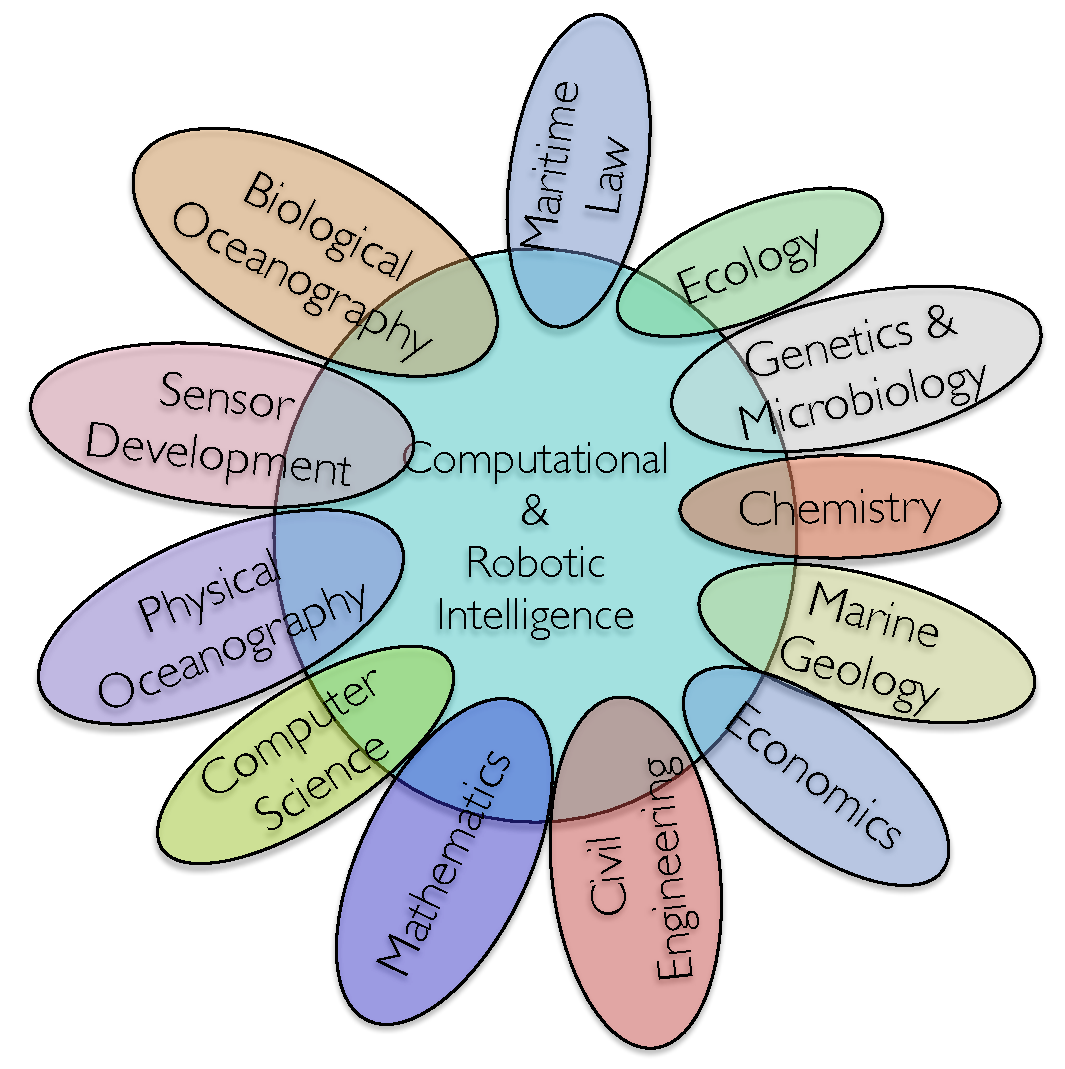
\includegraphics[scale=0.4]{fig/disciplines.pdf}
  \caption{The expectation of multi-disciplinary presentations for the
    \sympe. Given the intimate nature of the event, not all these
    fields would likely be represented.}
  \label{fig:concept}
  \vspace{-0.5cm}
\end{wrapfigure}

\vspace{+0.25in}

\noindent
We propose to hold a symposium with a novel format which brings
together a small ($\sim 30$ people) yet highly motivated group of
experts focusing on smarter methods in ocean observation.%  by leveraging
% developments in autonomous systems and computational intelligence.

Our primary aim of this symposium is to generate ideas across science
and technology with a central focus on computational and robotic
intelligence (Fig. \ref{fig:concept}).  In the process, we hope to
% have participants interact to 
make connections for ideation to advance observation methods at
various levels (national, international), during this \textsf{UN
  Decade of the Oceans}. By doing so, we hope for scientists to
understand and leverage advances in technology and for technologists
to advance their science and problem solving methods to have a real
societal impact. And together, to advance the state of ocean science
and our understanding of the worlds oceans.

While there is a general acceptance of the need for inter-disciplinary
efforts in the field and out of it, expertise continues to be siloed
and researchers tend to focus narrowly, missing out on integrative and
potentially more expansive efforts. This meeting is an attempt to
bringing people together in meaningful debate and interaction across
disciplinary, geographic and cultural boundaries, and do so in an
immersive, safe and thoughtful environment, where reaching out can
provide research dividends.

By interaction across disciplines, we imply those which ought to
occur, but rarely do; for instance an observational oceanographer with
a Statistician. Or a marine roboticist with a climate modeler. As a
result, our proposed \emph{by invitation only} symposium aims to be
different and meaningful in a number of ways:

\begin{itemize}

\item We expect people to present speculative and ``far-out'' yet
  grounded ideas/hypotheses/concepts which commingle with
  inter-disciplinary concepts, processes and actions. So for example,
  a biological oceanographer, speculating what it might take to get a
  measure of biodiversity within a volume of water, and how it might
  evolve with environmental variability. Or a roboticist trying to
  advance the state of online machine learning for a mobile platform
  to take measure of planktonic community structure using in-situ
  machine vision, as an example. 

\item We will pair each speaker with a 'commentator/critic' from a
  very different field who would be expected to reach into the
  speaker's ideas, shared \emph{a priori} to provide public feedback
  during the event. So a typical ``talk'' would be along the lines of:

  \begin{enumerate}

    \item 20 minutes -- Speaker presentation in some measure of
      detail and accessible to the audience
    \item 10 minutes -- Commentator, providing
      feedback/critique/comments/suggestions
    \item 5 minutes -- Speaker response/rebuttal

  \end{enumerate}

\item This is \emph{not} a talk-and-drop event, but participatory by
  design. So each participant will not only have an opportunity to
  present, but also play critic to someone. This also means the pace
  of the \symp will be more deliberate with adequate time for
  discussions, debates and networking, across \textbf{4 days}
  including a full day around a social/outdoor activity.

\item While this might be a considerable time commitment, one way we
  hope to attract the 'right' people is by having the event fully
  funded to cover air travel to/from Terceira, hotel stay, conference
  venue, all meals and social events. We estimate this to cost $\sim$
  US \$70K. Potential sponsors include:

  \begin{itemize}

  \item US Office of Naval Research (ONR)
  \item Research Council Norway (RCN)
  \item Regional govt. of Azores
  \item Portuguese Government
  \item Portuguese Foundation of Science and Technology (FCT)
  \item European Union networking funding (EU)

  \end{itemize}

\item One necessary condition for selecting participants therefore, is
  that they be able to ``stand on their feet'' and defend their ideas
  while articulating concepts in approachable terms i.e. limiting
  jargon and focusing on first principles. Listening to others while
  also being persuasive would be an important trait in those
  attending. Equally we \emph{do not expect} to have people who are
  reticent. Attributes we think would be critical for a participant in
  other words would be (in no particular order):

  \begin{itemize}

  \item being articulate
  \item engaging
  \item knowledgable as well as expository
  \item open to concepts well outside their comfort zone
  \item can challenge and debate with peers as well as those more
    seasoned without crossing an 'annoyance' boundary

  \end{itemize}

\end{itemize}  

\noindent
Such approaches in interaction, have long been used in Cognitive
Science and applied by one of us (Rajan) when founding the \nas
Workshop of Planning and Scheduling (a niche sub-discipline within
AI). Panels and posters will of course be part of the program but the
critical nature of open interaction makes for a kind of back-and-forth
that cannot be preordained or scripted. And if designed properly, this
can lead to a truly interactive and participatory process. We have
also successfully used this approach in the maritime community in 2013
in Gran Canaria and both Eidsvik and Rajan collaborated in organizing
an event in Trondheim in
2018\footnote{\url{https://wiki.math.ntnu.no/ocean-analytics/start}},
which while participatory, was not as direct as what we're proposing
here. The more deliberative aspects of this proposed event are seeded
in early Computer Science conferences in the late 60's and 70's in
Asilomar, California as also the 'Gordon Research Conferences' in the
sciences, albeit in a more intimate environment.


\section{Proposed Program}
\label{sec:pgm}

\begin{figure}[!h]
  \centering
  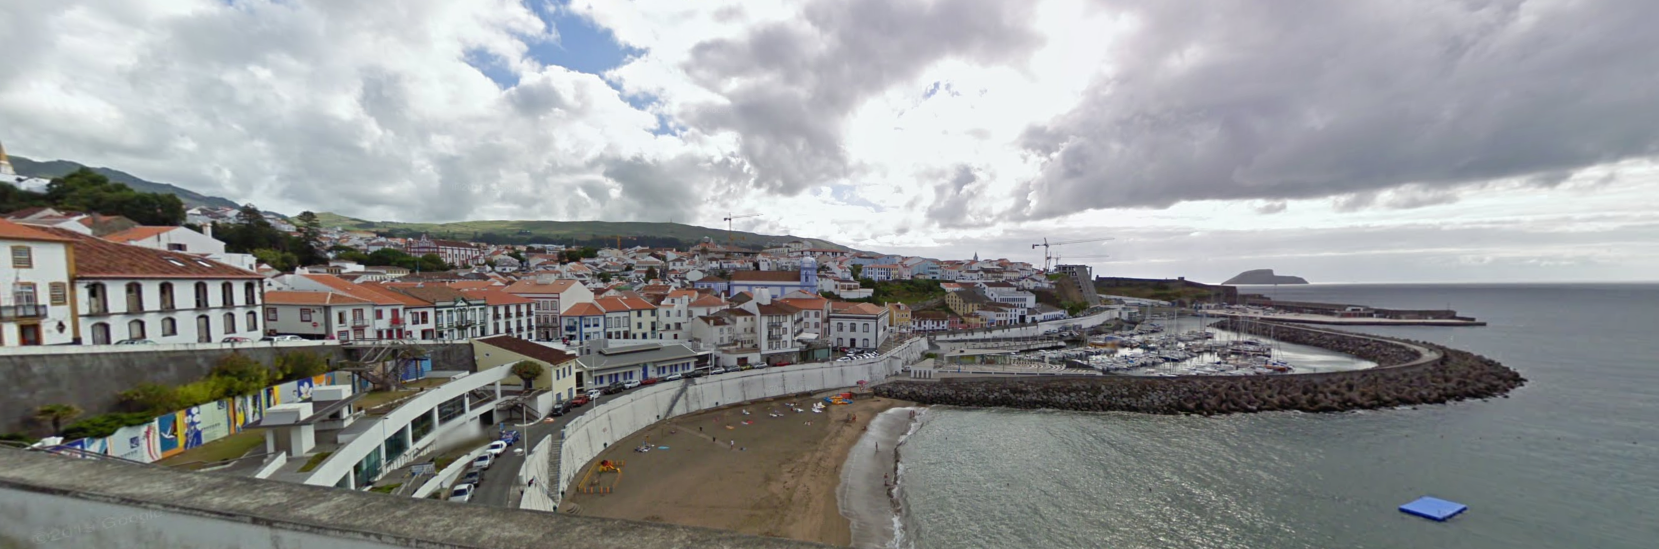
\includegraphics[scale=0.5]{fig/angra.png}
  \caption{\symp will be held in the picturesque town of Angra do
    Heroismo on Terceira Island, Azores.}
  \label{fig:angra}
\end{figure}

The \symp will be held on Terceira Island, in the Azores in the town of
Angra do Heroismo (Fig. \ref{fig:angra}). It houses the Lajes airfield,
which till recently was one of the largest military airfields outside
the US, run by the DoD and a strategic asset for long-distance
flights. Lajes is well connected to its neighboring islands, including
S\~{a}o Miguel, which enjoys direct connections to continental Europe
and to Boston and New York. Frequently run ferries also connect the
islands, although the pandemic has likely had an impact. The island
offers few distractions other than connecting with the ocean and to
nature, and therefore is an ideal setting for this event.

Angra itself is a picturesque small town and also houses the
headquarters of \aire~\footnote{\url{https://www.aircentre.org/}} which
will be the official host of the symposium. The Center will host a web
site with necessary information for the select attendees, and also
provide support during the event. A local organizer is already working
with the organizers to scout out potential hotel locations where all
attendees will be housed and will hold the meeting as well. 

\paragraph{Protocols \& timing} The \symp will be based on the
\texttt{Chatham House
  Rule}\footnote{\url{https://en.wikipedia.org/wiki/Chatham_House_Rule}}
and will require everyone to respect the ideas brought forth and not
take those ideas outside the meeting.  The organizers will ask all
attendees to be vaccinated prior to the event, with an European
Medicines Agency-approved vaccine and follow European Union protocols
at the time of the event.

Additionally, we are anticipating that the pandemic situation would
have eased or at least made in-person events less constraining by
early Summer (July) in 2022 and expect this event to be solely
in-person. Given the uncertain nature of the pandemic, we will target
this Spring/early Summer date, while keeping our options open to hold
it in the Fall, should there be unforeseen circumstances associated
with the pandemic. In large part, we are expecting stability in viral
caseload in holding the meeting at this time and doing so in-person
particularly because we value the person-to-person contact and
networking and the serendipitous connections expected, and one that
simply cannot replace a virtual event. The organizers will closely
monitor the situation prior and during the event, to ensure this event
is safe for all and focused on the science.

\begin{table}[!b]
  \centering
  % \vspace{-0.5cm}
  \begin{tabular}{|p{2.5cm}|p{2.5cm}|p{2.5cm}|p{2.5cm}|p{2.5cm}|}
    % \multicolumn{1}{l}{r}}{l}{l}
    \hline 
    \rowcolor{Gray}
    \bfseries Day 0& \bfseries Day 1&\bfseries Day 2 &\bfseries Day 3 &\bfseries Day 4\\
    \hline
                   &Morning Session 1&Morning Session 1&Morning Session 1&Morning Session 1\\
    \hline
                   &Coffee Break&Coffee Break&Coffee Break&Coffee Break\\
    \hline    
                   &Morning Session 2&Morning Session 2&Morning Session 2&Morning Session 2\\
    \hline
                   &Lunch&Lunch&Lunch&Lunch\\
    \hline
                   &Afternoon Session 1&Networking \& Outing&Networking \& Outing&Afternoon Session 1\\
    \hline
                   &Coffee Break&Networking \& Outing&Networking \& Outing&Coffee Break\\
    \hline
                   &Afternoon Session &Networking \& Outing&Networking \& Outing&Afternoon Session 1\\
    \hline
                   &Break&Networking \& Outing&Networking \& Outing&Break\\
    \hline
    Evening reception \& registration&Dinner&Outing \& Dinner&Outing \&
                                                               Dinner&Farewell Dinner\\
    \hline        
  \end{tabular}
  \caption{Proposed high-level program for the \sympe.}
  \label{tab:symp}
\end{table}

A proposed layout and schedule for the \symp is showing in Table
\ref{tab:symp}. The fundamental premise at this meeting is to connect a
diverse group of thinkers in academia looking at ways to make
oceanographic measurements and understand processes, to think 'out of
the box'. In-person networking is therefore crucial to this event. The
symposium expects to provide various venues to connect, both in the
formal presentation/challenge/rebuttal part, as also bonding over meals
and outdoors activities. We plan to offer all meals together, and urge
people to mix and network outside their traditional academic comfort
zones. The outings in particular will help the participants to connect
with nature especially the ocean which can easily be accessed on
Terceira. Coffee and snacks will eb available throughout the formal
session, and breaks will be frequent and well-paced to allow people to
connect. Relaxed meals will also offer the ability for conversations to
lead to synergistic ideas and concepts, we believe. This event is not
meant to be a traditional 'talk-and-drop' but targeted towards
engagement. 

\newpage
\section{Organizer's bios}
\label{sec:bios}


\parbox{6.5in}{
\begin{wrapfigure}{r}{3.6in - .75\columnsep} %{3.8in}{0.45\textwidth}
  % \centering
    \vspace{-\intextsep}
    \hspace*{-.35\columnsep}\includegraphics[scale=0.055]{fig/aida_snow_s.png}
\end{wrapfigure}
\textbf{Aida Alvera-Azcárate} is a researcher at the GeoHydrodynamics
and Environment Research (GHER) group of the University of Li\`{e}ge
(Belgium). She is a physical oceanographer specialising in the
development of data analysis techniques for ocean remote sensing, like
the gap-filling technique DINEOF (DataInterpolating Empirical Orthogonal
Functions), widely used by oceanographers. She also enjoys studying the
ocean dynamics from remote sensing data and the influence of ocean
dynamics on the ecosystem. She is Associate Editor of Remote Sensing of
Environment.\\

\textbf{email: }\emph{a.alvera@uliege.be}\\
\textbf{Web: }\url{http://labos.ulg.ac.be/gher/aida}
}

\vspace{20mm}

\parbox{6.5in}{
\begin{wrapfigure}{r}{3.6in - .75\columnsep} %{3.8in}{0.45\textwidth}
  % \centering
    \vspace{-\intextsep}
    \hspace*{-.35\columnsep}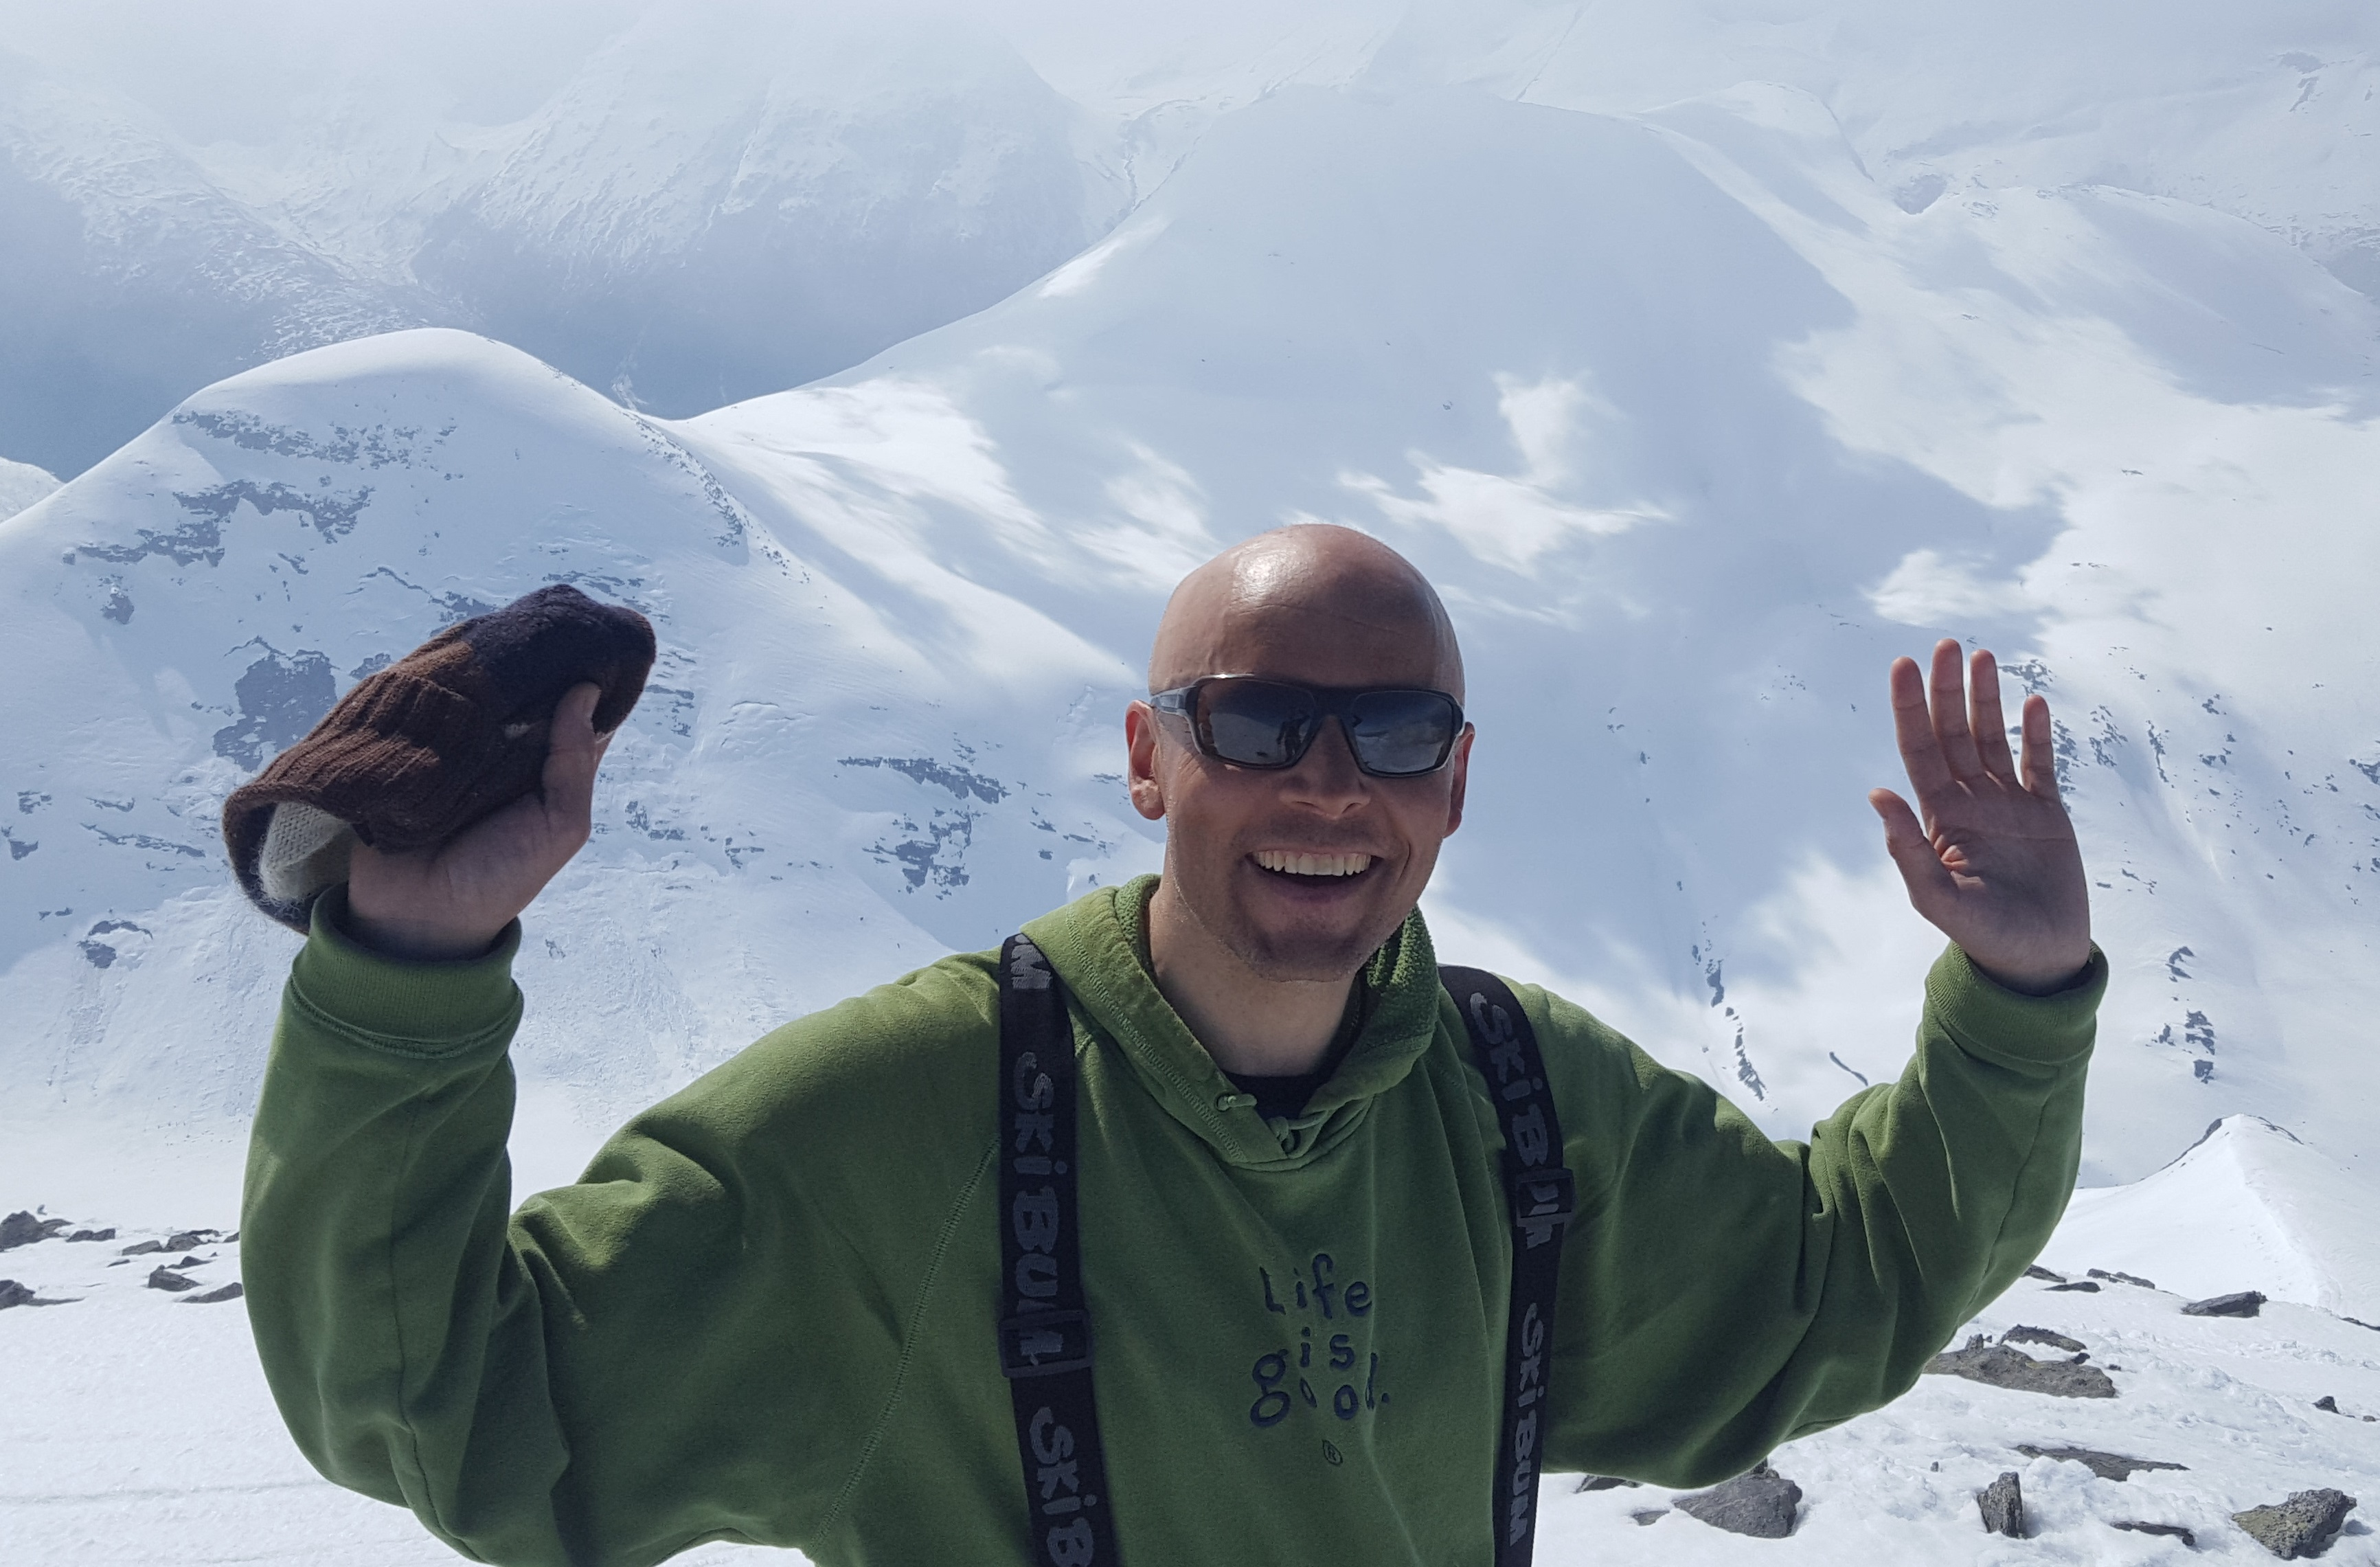
\includegraphics[scale=0.055]{fig/Eidsvikpicture.jpg}
\end{wrapfigure}
\textbf{Jo Eidsvik} is a Professor of Statistics at NTNU, Norway. His
research profile is in spatial and computational statistics applied to
the Earth sciences. He co-authored the book on Value of Information in
the Earth Sciences (Cambridge Univ Press, 2015). He has industry
experience from the Norwegian Research Defense Establishment and from
Equinor. He is currently involved in several research projects on
spatial and spatio-temporal modeling and monitoring, including ongoing
work on autonomous maritime sampling and a center for geophysical
forecasting.\\


\textbf{email: }\emph{jo.eidsvik@ntnu.no}\\
\textbf{Web: }\url{https://www.ntnu.no/employees/jo.eidsvik} }

\vspace{20mm}


\parbox{6.5in}{
\begin{wrapfigure}{r}{3.6in - .75\columnsep} %{3.8in}{0.45\textwidth}
  % \centering
    \vspace{-\intextsep}
    \hspace*{-.35\columnsep}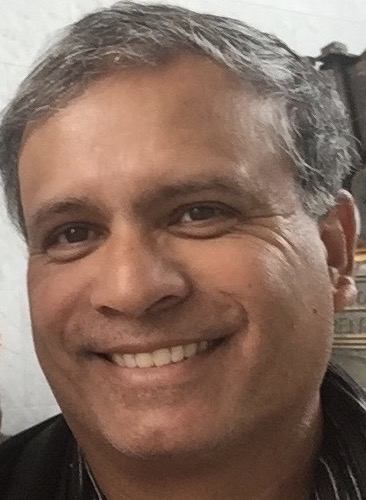
\includegraphics[scale=0.4]{fig/KRajan.jpg}
\end{wrapfigure}
\textbf{Kanna Rajan} is a Fellow at SIFT LLC and holds a visiting
faculty Professorship at \unive, Portugal in autonomous systems. At
\nas his software was responsible for the command/control of the 1999
New Millennium Deep Space 1, 65 Million miles from Earth and the 2003
Mars Exploration Rovers mission on the Red Planet. In 2005 he moved to
\mba to build the only AI group in marine robotics and to focus on
using machine intelligence for marine robotics and biological
oceanography.  His publications have been in highly ranked
peer-reviewed publications while his field work includes scientific
oceanographic cruises in the Pacific and the Atlantic. He will be a
Fulbright Fellow in Portugal in Spring 2022.\\

\textbf{email: }\emph{Kanna.Rajan@fe.up.pt}\\
\textbf{Web: }\url{https://kanna.rajan.systems}
}


\renewcommand{\thepage}{}
\end{document}